% !TEX encoding = UTF-8 Unicode
\chapter{Desarrollo experimental}

%\markboth{Desarrollo experimental}{}

%Como se mencionó en la sección anterior, el sensor utilizado posee un sistema de medición \textcolor{red}{sigue sin quedar claro - ¿sistema de que?)} ortogonal de 3 ejes. 
%En el cual cada uno recopila datos de aceleración a lo largo de cada una de las direcciones en las que está dirigido, de manera que la información registrada sobre cada eje es independiente de la generada en los 2 restantes.\textcolor{red}{no se entiende la frase, sugiero recortar} 
%Se consideró que estas características son suficientes para obtener la información necesaria para el estudio de la dinámica de un vehículo.

Como se mencionó en la sección anterior, el sensor utilizado posee un sistema de medición ortogonal de tres ejes.
Cada uno recopila datos de aceleración a lo largo de la dirección en la que está dirigido. 
De manera que la información registrada sobre cada eje es independiente de la generada en los dos restantes.

Idealmente el sistema de ejes del sensor debe permanecer siempre fijo al vehículo, de tal manera que cualquier movimiento realizado por el vehículo sea igualmente realizado por el sensor. 
La configuración de ejes designada para el vehículo, a la cual se alineó el sensor de la forma más cercana posible, se describe a continuación: el eje $z$ es perpendicular al plano del suelo, el eje $x$ está dirigido a lo largo de la línea de movimiento principal del vehículo, siendo el eje $y$ perpendicular a los ejes $x$ y $z$. 
La configuración descrita se ilustra en la figura \ref{ejes}.

\begin{figure}[H]
\centering
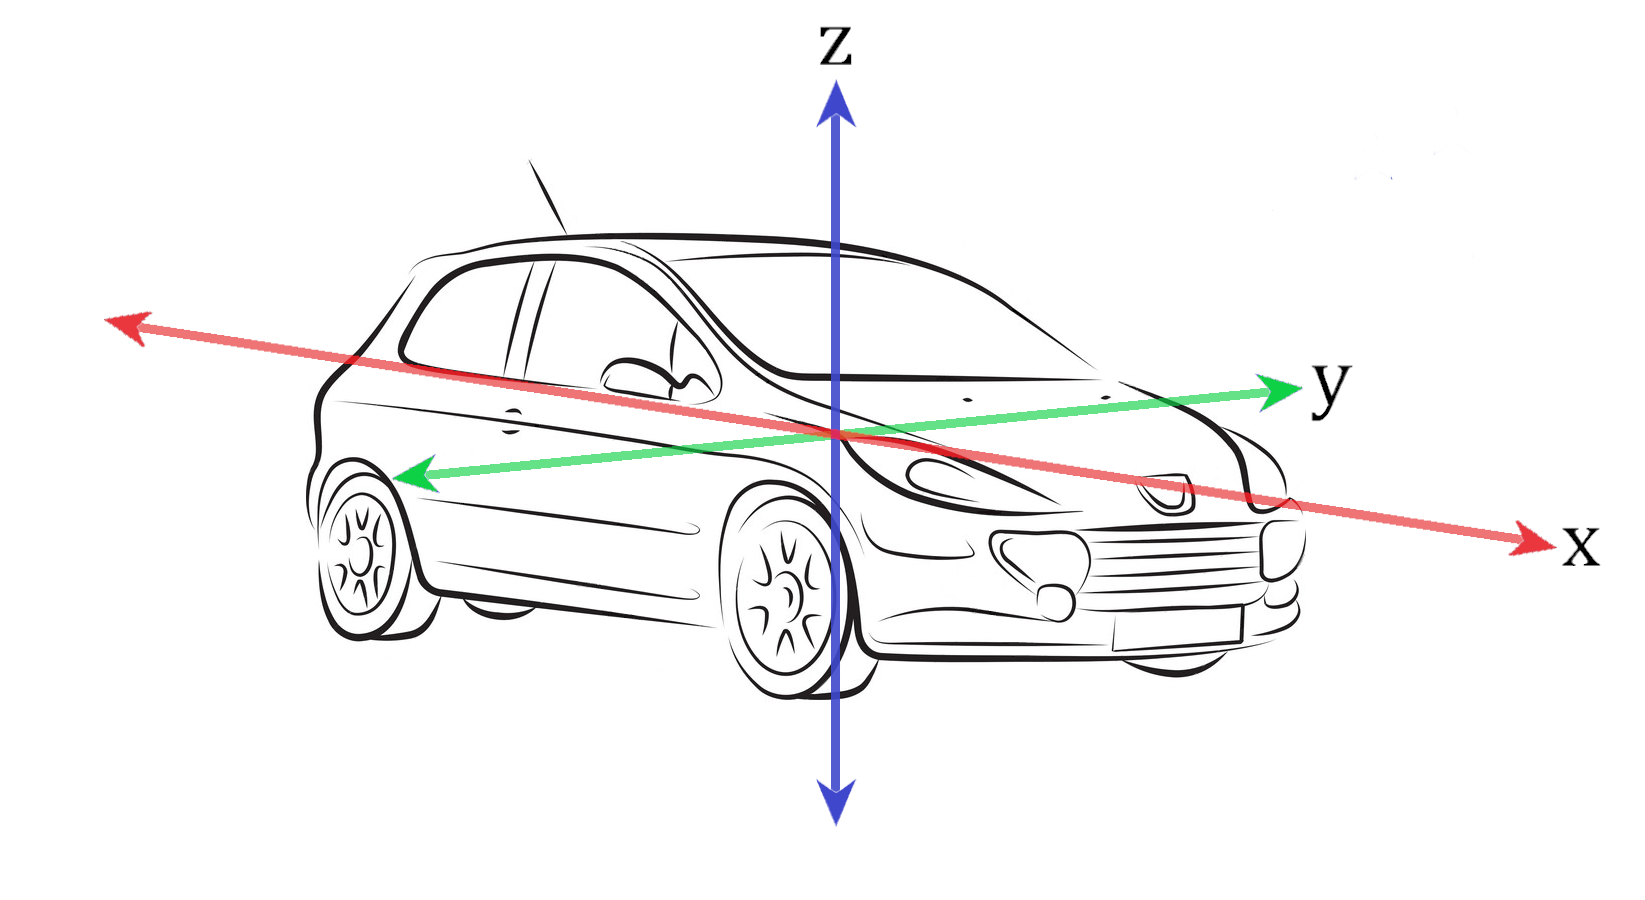
\includegraphics[scale=0.30]{car9.png}
\caption[Caption for LOF]{Sistema de ejes ortogonales\footnotemark[1].}
\label{ejes}
\end{figure}
\footnotetext[1]{Imagen modificada tomada de: https://www.vectorstock.com/royalty-free-vector/car-sketch-vector-98800}

Haciendo uso del equipo de medición, compuesto por el sensor de aceleración y el sistema GPS se realizaron diversas pruebas a bordo de un vehículo.

%\textcolor{orange}{(poner imagen del wiimote fijado al vehículo?)}\\

%El sensor fue colocado y alineado a la configuración de ejes antes mencionada\textcolor{red}{sigue igual (esto ya lo dijiste es redundante)}. 
%Una vez encendido, el sensor era identificado de manera inalámbrica por una computadora a bordo del vehículo, a la cual le transmitía los datos de aceleración de la misma manera, por medio de tecnología Bluetooth \textcolor{red}{si es por bluetooth ya es inalámbrico, sobra decirlo}. 

Una vez encendido, el sensor se comunicaba con una computadora a bordo del vehículo por medio de la tecnología Bluetooth, a la cual le transmitía los datos de aceleración.
Complementariamente se utilizó un dispositivo con GPS como apoyo para visualizar la trayectoria que se recorrería, con el fin de tener una mejor idea de cómo podría afectar la geometria de la ruta a las mediciones obtenidas por el sensor inercial a bordo del vehículo.

Para cada uno de los tres eventos (definidos en la primera sección) se designó una {\em etiqueta} con el propósito de diferenciarlos entre sí.
La etiqueta consistía en un carácter, diferente para cada evento, que el algoritmo registraba junto a los datos del evento correspondiente, cuando este tomaba lugar. 
Esta discriminación únicamente servía de ayuda al usuario para identificar más fácilmente los datos relativos a cada forma de conducir.

Adicionalmente se establecieron otras dos etiquetas para la obtención de datos, las cuales correspondían a una conducción regular y a una condición en la que el vehículo permanecía estático, pero con el motor encendido.
 
\section{Vehículo estático}

Lo primero en realizarse fue un registro de datos destinado únicamente para la etiqueta {\em vehículo estático}. 
Esto simplemente consistió en dejar el vehículo encendido y sin moverse en una superficie plana horizontal, por un lapso de $22s$.
Lo anterior se realizó con el objetivo de estudiar el espectro de frecuencias correspondiente a la señal obtenida por el sensor, buscando la posible presencia de algunas frecuencias con una amplitud significativa, esto es, superior a las demás. 
De ser así, dichas frecuencias corresponderían a las frecuencias fundamentales de vibración del motor, las cuales serían una fuente de ruido que perturbaría la exactitud de las mediciones de aceleración del vehículo. 
Durante el periodo de obtención de datos se verificó que el sensor se mantuviera fijo a la superficie a la que se adhirió, sin sufrir ningún tipo de deslizamiento, giro o desprendimiento de esta.

\section{Conducción regular}

El primer recorrido para el que se realizaron mediciones de aceleración fue el dedicado a la conducción regular. 
El cual consistió en conducir el vehículo de una manera conservadora, sin realizar ningún movimiento fuera de lo normal, a una velocidad de aproximadamente $80 km/h$ (dicha velocidad se considerará en adelante como el valor de {\em velocidad regular}).
Este recorrido tuvo una duración de aproximadamente $115 s$. %y consistió en conducir el vehículo en línea recta, en una superficie plana horizontal, a una velocidad regular, manteniéndolo lo más estable posible.

La conducción fue realizada sobre una superficie plana horizontal; y la ruta a seguir, tanto para este como para los posteriores recorridos, constaba de tramos rectos con algunas curvas suaves entre ellos, como se puede apreciar en la figura \ref{ruta} $b)$.\\
\pagebreak

\begin{figure}[H]
\begin{textblock*}{190mm}(5cm,7.5cm)
$a)$

\vspace{6.8cm}

$b)$
\end{textblock*}
\centering
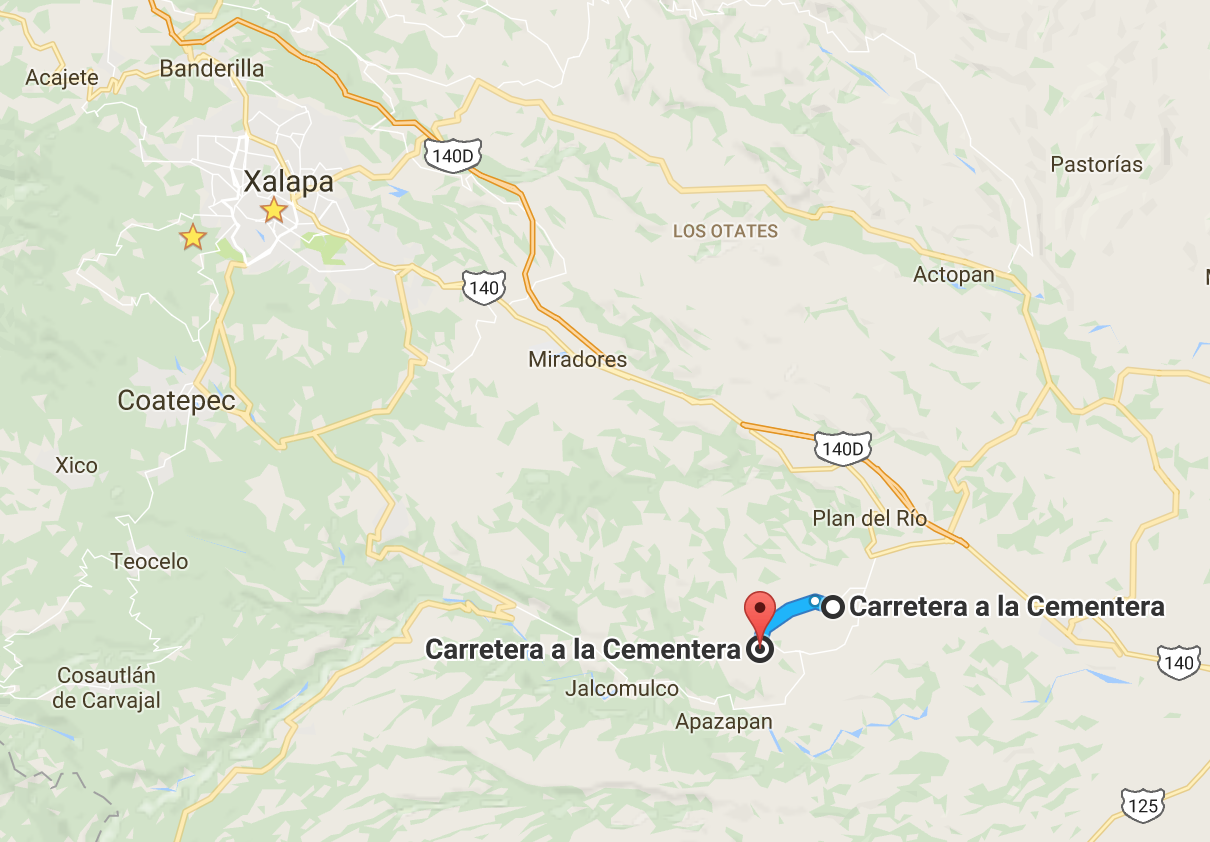
\includegraphics[scale=0.49]{Captura2.png}

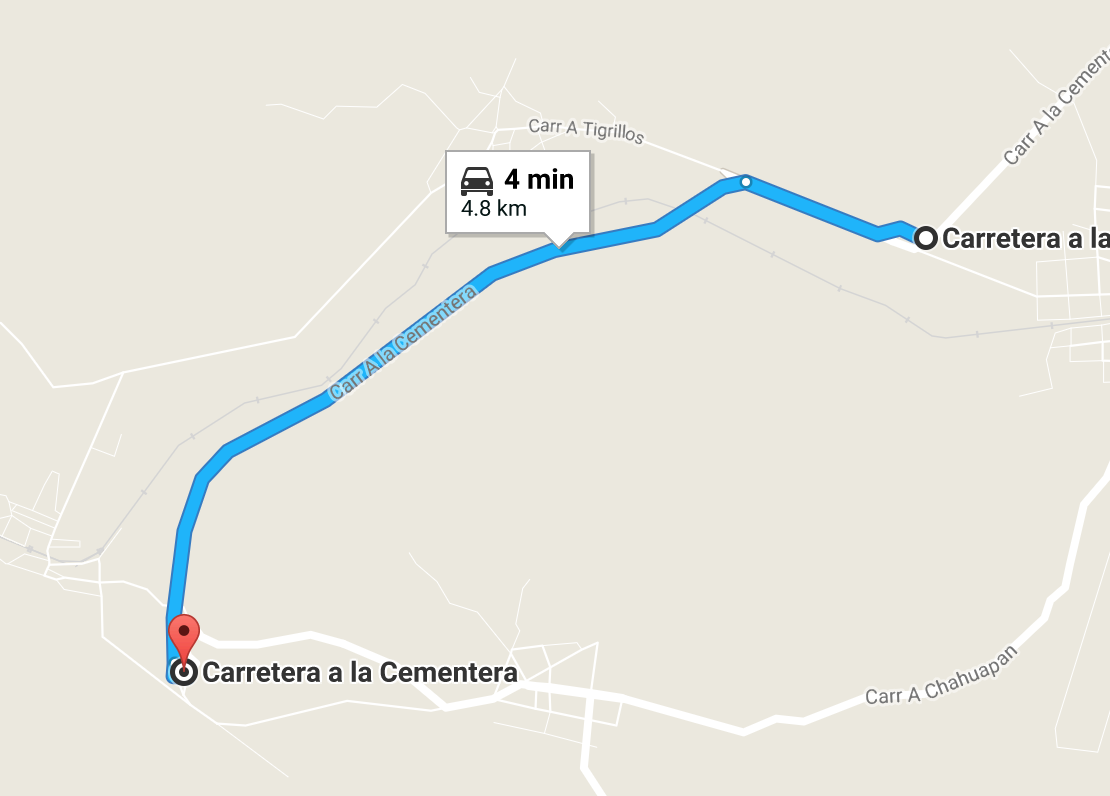
\includegraphics[scale=0.534]{Captura1.png}
\caption{$a)$ Ubicación de la ruta. $b)$ Ruta recorrida.}
\label{ruta}
\end{figure}

La recopilación de los datos para el modo de conducción regular se realizó con la finalidad de analizar el espectro de frecuencias de su señal y compararlo con el de los demás eventos. 
Esto para verificar que los espectros de frecuencias de los eventos detectables tuviesen características distintas a los de una conducción regular. 
Ya que, de no presentarse características suficientes para diferenciar los espectros de frecuencias de una conducción regular con respecto a los correspondientes a eventos, esto causaría problemas para discriminarlos entre sí analíticamente. 
Además, se verificó que no hubiese registros fuera de lo ordinario en la señal obtenida durante el recorrido; lo cual, de ser así, sería indicativo de alguna falla en los dispositivos utilizados.

Luego de obtener los datos correspondientes al vehículo estático y a una conducción regular, los cuales tendrían un papel complementario en el análisis, se inició con la recopilación de las señales asociadas a los eventos que se deseaban detectar.

\section{a) Evento de frenado}

El segundo recorrido realizado fue el dedicado al evento de frenado, el cual tuvo una duración total de $234s$ y consistió en varias conmutaciones entre conducciones regulares y eventos de frenado. 

Durante el trayecto se realizaron cuatro eventos de frenado, comenzando con una conducción regular. 
Se avanzó a la velocidad regular correspondiente, en la cual se evitó realizar cualquier movimiento anómalo que dificultara el posterior análisis.

Después haber transcurrido aproximadamente $84s$ de conducción regular se realizó el primer evento de frenado. 
Se frenó en un periodo de tiempo de aproximadamente $3s$, de manera que el vehículo quedó completamente detenido. 
Después de haber frenado al vehículo se comenzó a acelerar hasta recuperar la velocidad regular. 
Una vez que se había alcanzado la velocidad deseada se dio por culminado el evento de frenado, dando lugar a la conducción regular nuevamente. 
Desde que el vehículo comenzó a frenar hasta terminar el evento transcurrieron $15s$.

Los tres eventos de frenado restantes se realizaron de forma similar al primero. 
Los eventos que tuvieron mayor duración de los cuatro tardaron $18$ y $19s$ en llevarse a cabo, mientras que los dos restantes se ejecutaron en un periodo de $15s$ aproximadamente.

Todos los eventos de frenado que se realizaron durante este recorrido trataron de efectuarse de manera que fueran lo más parecidos posible entre sí, con la finalidad de que el patrón correspondiente a su dinámica quedara bien establecido, para que de esta forma su detección no presentara mayores dificultades. 
Todos los frenados se realizaron mientras el vehículo avanzaba en línea recta, los tramos curvos se asignaban a la conducción regular.

\section{b) Evento de rebase}

Después de haber recopilado los datos correspondientes al recorrido en el que se ejecutaron los eventos de frenado, se procedió a realizar otro recorrido, el cual estaría enfocado en capturar datos del evento rebase.

El recorrido dedicado al evento de rebase tuvo una duración total de $173s$, durante los cuales, al igual que con el evento de frenado, se cambió entre el modo de conducción regular y el evento de rebase en varias ocasiones. 

Se realizaron un total de tres eventos de rebase para este recorrido, comenzando con un tramo de conducción regular, seguido del primer evento de rebase. 
Para lo cual el piloto realizó la maniobra de un rebase común; aumentando la velocidad hasta un valor por encima de la velocidad regular, de aproximadamente $100km/h$, al mismo tiempo que desplazaba al vehículo hacia el carril adyacente de una manera moderada. 
Luego se avanzó durante algunos segundos sobre este carril, para posteriormente incorporarse de nuevo al carril de transito normal respectivo, de forma igualmente moderada. 
Después de lo cual se comenzó a reducir la velocidad hasta recuperar la que se tenía antes de ejecutar el rebase. 
Con esto se dio por finalizado el evento de rebase y se pasó al modo de conducción regular nuevamente. 
El primer evento de rebase para este recorrido duró un total de $19s$.

Los dos eventos de rebase siguientes se llevaron a cabo en forma semejante al primero, siendo de 20 y $16s$ los de mayor y menor duración.
Todos los rebases fueron hechos en tramos rectos y prácticamente horizontales, las trayectorias curvas se condujeron en modo de conducción regular.

\section{c) Evento de movimiento en zig-zag}

Luego de la recopilación de los datos correspondientes a los eventos de rebase y de frenado se llevó a cabo el recorrido dedicado al evento de movimiento en zig-zag. 
%Este recorrido tuvo una duración total de aproximadamente 265 segundos, durante los cuales se realizaron 4 eventos de zig-zag más un evento extra de rebase \textcolor[rgb]{1,0,0}{(esto es irrelevante)}. 
%El evento de rebase fue realizado con la finalidad de tener un número igual de muestras para cada tipo de evento, ya que tanto en el recorrido del evento de frenado como en el de zig-zag se realizarían 4 eventos en total. 
%Entonces, para efectuar un mejor análisis, se decidió aumentar el número de muestras añadiendo otro evento de tipo rebase.
Este recorrido tuvo una duración total de aproximadamente $265s$, durante los cuales se realizaron cuatro eventos de zig-zag y uno de rebase.

El recorrido consistió, al igual que los anteriores, en cambios entre conducción regular y los eventos que se querían detectar (zig-zag y rebase para este caso). 

Se inició el recorrido partiendo de una conducción regular, alcanzando una velocidad de $80km/h$.
El primer evento de movimiento en zig-zag se realizó después de este periodo; consistió en mover al vehículo de izquierda a derecha sobre el eje $y$ en repetidas ocasiones, usando el ancho de la pista. 
La frecuencia con la que se realizaban las oscilaciones era relativamente elevada, tratando de simular lo más parecido posible el caso real de un evento de tales características, en el que no se tiene el suficiente control del vehículo.

El evento de movimiento en zig-zag finalizó al dejar de realizar los movimientos de un lado a otro e incorporarse lentamente al carril correspondiente. 
Este evento tuvo una duración de $11s$, durante el cual se realizaron tres oscilaciones.

Los tres eventos de movimiento en zig-zag restantes fueron ejecutados de forma análoga al primero, con la diferencia de que tuvieron diferente número de oscilaciones: efectuando cuatro oscilaciones para el segundo, cinco para el tercero y seis para el cuarto; siendo este último el de mayor duración con $23s$.
Los tiempos de duración de los eventos fueron directamente proporcionales al número de oscilaciones.

El evento de rebase realizado en este recorrido tuvo una duración de aproximadamente $10s$. 
El cual se realizó imitando de la manera más parecida posible, las características de los rebases realizados en el recorrido dedicado a estos eventos.

Todos los eventos correspondientes a los movimientos en zig-zag, al igual el evento de rebase, se realizaron a lo largo de trayectos rectos, prácticamente horizontales y sin ninguna imperfección importante sobre el camino que pudiera representar un problema para el análisis o la adquisición de datos. 
Los tramos curvos se recorrieron en modo de conducción regular.

\section{Recorrido para validación}

Por último se realizó un recorrido adicional, en el cual se ejecutaron los tres eventos que se deseaban detectar: el frenado, el rebase y el movimiento en zig-zag. 
Esto con el fin de tener un conjunto de datos al cual posteriormente someter a una prueba de detección de los eventos de interés. 
Con el propósito de corroborar que los métodos empleados en la detección de tales eventos funcionasen de manera correcta, y de ser así, cumplir con el principal objetivo de este trabajo.

El recorrido consistió en ejecutar una vez cada uno de los tres eventos mencionados anteriormente. 
Antes y después de cada evento detectable se estableció la realización del tipo de pilotaje correspondiente a una conducción regular. 
Esto con la finalidad de que, al someter los datos a las pruebas de detección, el algoritmo pudiera diferenciar entre este tipo de conducción y los eventos que se esperaba fueran detectados.

En total, este recorrido tuvo una duración de $142s$.
Se inició el recorrido manejando el vehículo de una manera moderada, correspondiente a una conducción regular.

El primer evento en ejecutarse fue el movimiento en zig-zag, el cual consistió en mover el vehículo sobre el eje $y$, tal y como se describió en la sección dedicada a este evento.
El evento finalizó al dejar de realizar oscilaciones sobre el eje $y$, realizando un total de cinco oscilaciones. 
La duración de este evento fue de $17s$ y durante su ejecución se procuró que las características del evento fueran lo más parecidas posibles a los eventos de zig-zag realizados anteriormente.

El segundo evento detectable del recorrido fue el evento de frenado, el cual tuvo una duración de $17s$, durante los cuales se ejecutó la maniobra imitando las características de los eventos de frenado realizados anteriormente.

El último evento efectuado en este recorrido fue el evento de rebase, cuya ejecución tardó $14s$. 

%Los eventos realizados en este recorrido se llevaron a cabo sobre trayectos rectos y horizontales, los cuales no presentaban irregularidades que afectaran la conducción deseada o la correcta recopilación de datos. 
%Los trayectos curvos fueron recorridos durante los intervalos de tiempo en los que se efectuó la conducción regular.

Con la culminación de este recorrido se dio por terminada la recopilación de datos. 
Se decidió que se tenían las muestras suficientes para realizar un análisis adecuado en busca de los resultados deseados.
La información de cada recorrido se resume en la tabla \ref{tablarecorridos}.\\

\renewcommand{\arraystretch}{1.5}

\begin{table}[H]
\centering
\begin{tabular}{>{\centering\arraybackslash} m{4cm}|>{\centering\arraybackslash} m{2cm}|>{\centering\arraybackslash} m{2.5cm}|>{\centering\arraybackslash} m{2.7cm}}
%\toprule[1.2pt]
\hline \hline
\bf Nombre del recorrido o prueba & \bf Duración total & \bf Eventos realizados & \bf Duración de 
cada evento \\ 
\hline \hline 
%\Gape[1cm][1cm]
%\addlinespace
%\midrule
Vehículo estático & $22\ s$ & Ninguno & - \\ \hline
%\midrule
Conducción regular & $115\ s$ & Ninguno & - \\ \hline
%\midrule
\multirow{4}{*}{Frenado} & \multirow{4}{*}{$234\ s$} & $1^\text{er}$ Frenado & $15\ s$ \\ \cline{3-4}
& & $2^\text{o}$ Frenado & $19\ s$ \\ \cline{3-4}
& & $3^\text{er}$ Frenado & $15\ s$ \\ \cline{3-4}
& & $4^\text{o}$ Frenado & $18\ s$ \\ \hline
%\midrule
\multirow{3}{*}{Rebase} & \multirow{3}{*}{$173\ s$} & $1^\text{er}$ Rebase & $19\ s$ \\ \cline{3-4}
& & $2^\text{o}$ Rebase & $16\ s$ \\ \cline{3-4}
& & $3^\text{er}$ Rebase & $20\ s$ \\ \hline
%\midrule
\multirow{5}{*}{Movimiento en zig-zag} & \multirow{5}{*}{$265\ s$} & $1^\text{er}$ Zig-zag & $11\ s$ \\ \cline{3-4}
& & $1^\text{er}$ Rebase & $10\ s$ \\ \cline{3-4}
& & $2^\text{o}$ Zig-zag & $15\ s$ \\ \cline{3-4}
& & $3^\text{er}$ Zig-zag & $19\ s$ \\ \cline{3-4}
& & $4^\text{o}$ Zig-zag & $23\ s$ \\ \hline
%\midrule
\multirow{3}{*}{Recorrido para validación} & \multirow{3}{*}{$142\ s$} & $1^\text{er}$ Zig-zag & $17\ s$ \\ \cline{3-4}
& & $1^\text{er}$ Frenado & $17\ s$ \\ \cline{3-4}
& & $1^\text{er}$ Rebase & $14\ s$ \\
\hline \hline
%\bottomrule[1.2pt]
\end{tabular}
\caption{Información más relevante de cada recorrido.}
\label{tablarecorridos}
\end{table}

En este capítulo se describieron las condiciones en las que se llevaron a cabo las mediciones para esta investigación.
%\textcolor{blue}{Como comentario final de este capítulo se puede puntualizar que las condiciones en las que se llevaron a cabo las mediciones para esta investigación fueron las idóneas para su realización.
Todos los recorridos se realizaron sobre la misma ruta. 
No se presentaron problemas por parte del vehículo o del equipo de cómputo utilizado. 
Además de que la alineación y correcta obtención de datos por parte del equipo de medición (acelerómetro y GPS) fueron cuidadas a lo largo de los recorridos.
En el siguiente capítulo se describirá el análisis realizado con estos datos.
